\documentclass{jsarticle}
\usepackage{amssymb}
\usepackage{graphicx}
\usepackage[dvipdfmx]{color}
\usepackage{here}
\usepackage{tabularx}
\usepackage{amsmath}
\usepackage{amsthm}
\usepackage{url}
\usepackage[hang,small,bf]{caption}
\usepackage[subrefformat=parens]{subcaption}
\usepackage{tikz}
\usepackage{siunitx}
\usepackage{bm}
\usepackage{ascmac}
\usepackage[top=15truemm,bottom=20truemm,left=20truemm,right=20truemm]{geometry}
% \usepackage{fancybx}
\usetikzlibrary{shapes.geometric}
\usetikzlibrary {shapes.misc}
\usetikzlibrary{positioning}
\captionsetup{compatibility=false}


\begin{document}
4/21

\section*{Ex3.6}
問題文\\
\begin{equation}
  \dot x = f(t,x)\;,\;x(t_0) = x_0 \tag{3.1}
\end{equation}
$f(t, x)$を、$t$について区分的に連続であり、
$x$について局所リプシッツであり、
\begin{equation*}
  \left\|f(t, x)\right\|\leq k_1 + k_2\left\|x\right\|, (t, x)\in [t_0,\infty)\times \mathbb{R}^n
\end{equation*}
を満たすとする。

(a)(3.1)の解が存在するすべてのtに対して次式を満たすことを示せ。
\begin{equation*}
  \left\|x(t)\right\|\leq \left\|x_0\right\|\exp\left[k_2(t-t_0)\right]+\frac{k_1}{k_2}\{\exp\left[k_2(t-t_0)\right]-1\}\;,\;\forall t\geq t_0
\end{equation*}

(b) その解は有限の脱出時間を持つことができるか。

\vspace*{1cm}

解答

(a) 

(3.1)の解は以下のように書ける。
\begin{equation*}
  x(t) = x_0 + \int^t_{t_0} f(s,x) ds
\end{equation*}
$$
\begin{aligned}
  \|x(t)\| &\leq \|x(t_0)\| + \int_{t_0}^{t} \|f(s,x(s))\| ds \\
  &\leq \|x(t_0)\| + \int_{t_0}^{t} k_1 + k_2\|x(s)\| ds \\
  &\leq \|x(t_0)\| + k_1(t-t_0) + k_2 \int_{t_0}^{t} \|x(s)\| ds \\
  % &\leq \|x(t_0)\| \exp(k_2(t-t_0)) + \frac{k_1}{k_2} \left[ \exp(k_2(t-t_0))-1\right]
\end{aligned}
$$

Gronwall-Bellman inequality より、
$$
\begin{aligned}
  \|x(t)\|&\leq \|x(t_0)\| + k_1(t-t_0) + \int_{t_0}^{t}[\|x_0\| + k_1(s-t_0)]k_2 \exp\{k_2(t-s)\} ds 
\end{aligned}
$$
計算して、
\begin{equation*}
  \left\|x(t)\right\|\leq \left\|x_0\right\|\exp\left[k_2(t-t_0)\right]+\frac{k_1}{k_2}\{\exp\left[k_2(t-t_0)\right]-1\}\;,\;\forall t\geq t_0
\end{equation*}
が成り立つ。

(b) 解が有界でない場合、解は有限の脱出時間を持つ。
しかし、(a)で式(3.1)の解は有界であることが示されているため、解は有限の脱出時間を持つことができない。


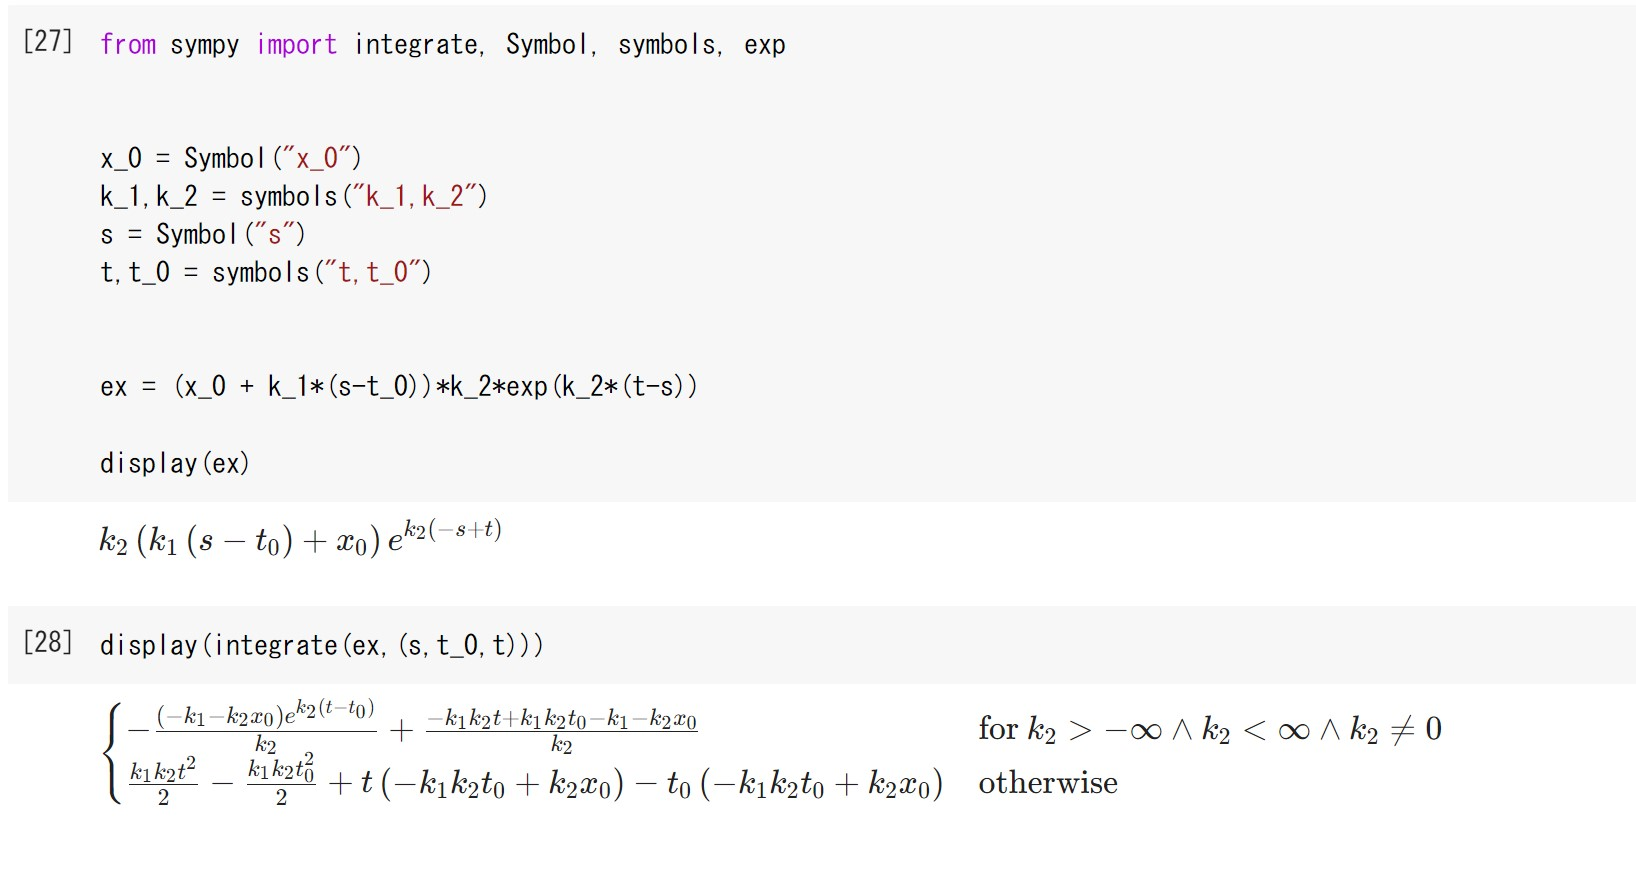
\includegraphics[width=15cm]{integral.jpg}

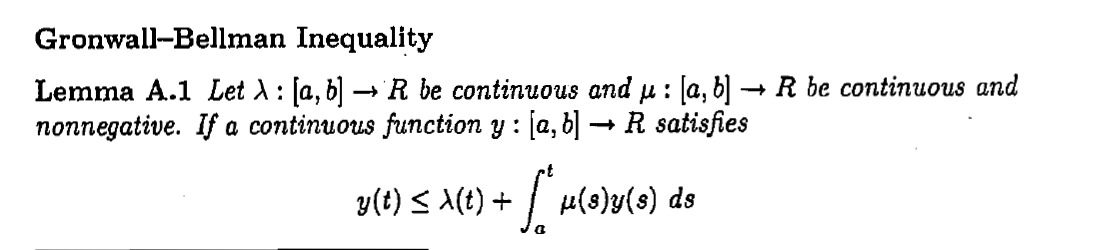
\includegraphics[width=15cm]{A.1_1.png}

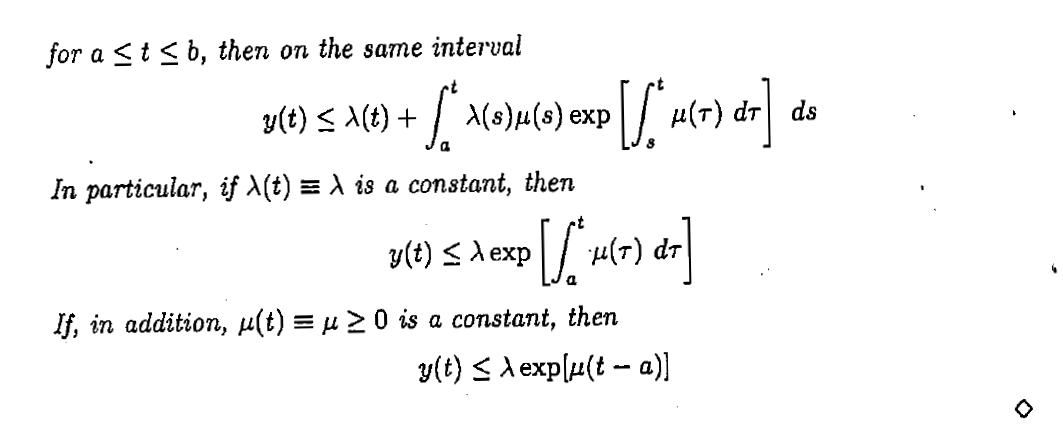
\includegraphics[width=15cm]{A.1_2.png}

\end{document}